\documentclass[../main.tex]{subfiles}
\begin{document}
\section{Improved Sea Lion Optimization (ISLO)}
\label{improved_ISLO}
	Sea Lion Optimization (SLnO) is one of the newest swarm-based optimization algorithm. In experiments in SLnO original paper \cite{masadeh2019sea}, SLnO is proved that it outperformed several well-known bio-inspired model such as Generic Algorithm (GA), Particle Swarm Optimization (PSO) and Whale Optimization Algorithm (WOA). However, like many other algorithms, SLnO also faces the problem of local minimum, slow convergence and diversity degradation of population. In SLnO's exploitation phase, the updating operation \ref{slno_eq2} only takes the distance between the current agent and the best solution into account, which makes updated position always oriented to one direction, leading to poverty of exploitation ability. Also, in exploration phase, although the participation of two agents that already exist in population in the updating operation \ref{slno_eq8} helps the new-born solution inherits current decent features of population, new solution has no way to reach another position outside of existing positions. This results in a dramatic decrease in the diversity of population, and significantly influences the ability of escaping local minimum of SLnO algorithm. All things considered, we decided to enhance those 2 operators by taking individual information into account for exploitation phase, and using a technique called opposition-based operation for exploration phase. These two improvements form a new version of SLnO called Improved Sea Lion Optimization (ISLO) algorithm. The pseudo code of the algorithm is presented in Algorithm \ref{algorithm_islo}, and  our improvements would be discussed in detail in \ref{imprv_exploit} and \ref{imprv_explore} as below.  
\begin{algorithm}[!t]
\caption{Improved Sea Lion Optimization (ISLO)}
\label{algorithm_islo}
\SetAlgoLined
 Initialize the Sea Lion population $X_i (i=1,2,.., n)$ randomly. \\
 Calculate fitness of each solution (sea lion). \\
 $X_*\gets$ the best solution \\
\For {$Iter=0 \to Iter_{max}$}{
	Calculate the value of $C$ \\
	\For {SeaLion in population}{\
		Calculate $SP_{leader}$ using Eq. \ref{snlo_eq3}  \\
		\uIf{$SP_{leader} < 0.25$}{
			\uIf {$|C| < 1$}{\
				Calculate $Dist_1$ and $Dist_2$ using Eq. \ref{islo_eq1} and \ref{islo_eq2}
				Update the location of the current search agent using Eq. \ref{islo_eq3}
				}
			\Else {
				Choose a random search agent $SL1_{rand}$ and $SL2_{rand}$ \\
				Update the location of current search agent by Eq. \ref{islo_eq6} \\
			}
		}	
		\Else{
			Update the location of the current search agent by Eq. \ref{slno_eq6}
		}
	Evaluate population: fix if any solutions go beyond the boundary \\
 	Recompute the fitness of all solutions \\
 	Check and update $X_*$ if a better solution is found. \\
	}

}
 \textbf{Results:}  $X_*, f(X_*)$
\end{algorithm}
   
\subsection{Exploitation phase improvement}
\label{imprv_exploit}
	As mentioned above, SLnO have its own drawbacks in its exploitation phase. In order to enhance the performance of the operation \ref{slno_eq2}, not only distance between the current agent and the best agent, but also the influences of an individual experiment in history is considered in new improved operation. This idea stems from the updating mechanism of PSO \cite{eberhart1995particle} where the velocity of a particular particle is influenced by both the best individual and best personal information. This combination can take advantages of both the intelligence of the whole swarm and of each individual, and therefore there is more information for agents to exploit, leading to more potential exploitation capability of algorithms. 
	
	Following that idea, we apply the information sent from best individual experiment in the same way as best agent position. The formulas of new updating mechanism for exploitation phase is as follows:
\begin{equation}\label{islo_eq1}
Dist_1 = |2B.P(t) - SL(t)| 
\end{equation}
\begin{equation}\label{islo_eq2}
Dist_2 = |2B.P_i(t) - SL(t)| 
\end{equation}
\begin{equation}\label{islo_eq3}
SL(t+1) = c_1r_1(P(t) - Dist_1.C) + c_2r_2(P_i(t) - Dist_2.C)
\end{equation}
where $P_i(t)$ is the personal best position of agent $i$ up to time $t$, $c_1$, $c_2$ 2 are positive constant parameters called acceleration coefficients and $r1, r2$ are random numbers in range $[\, 0,1 ] \,$.

	In new operation \ref{islo_eq3}, the new-updated position of an individual is the result of adding two vectors, one is the vector presenting the direction of that individual towards the best agent, and another is the direction towards its own experiences in history. The influences of both two factors are determined by two random numbers $r_1$ and $r_2$. $r_1$ and $r_2$ play an extremely important role in the updating mechanism,  because  they create random characteristics for the operation, helping ISLO avoiding local minimum and taking advantages of the two factors. Without the appearance of $r_1$ and $r_2$, the updated position is always affected exactly half by best agent and half by its experience, which may lead to degradation of the diversity of population. 

\subsection{Exploration phase improvement}
\label{imprv_explore}
	
	In original SLnO algorithm, new-born agents that are created in exploration phase cause a poor exploration search ability because of inheriting features of existing solutions. In order to tackle this problem, exploration phase is required the operation to have the ability of creating a decent new-born solution. New updated position need to satisfy two characteristics: carrying random features for ensuring a strong capability of exploration phase, and landing in a position decent enough (close enough to the best agent position) for updating positions in the next generation. From that motivation, a method called Opposition-based Learning (OBL) \cite{tizhoosh2005opposition}, which is successfully applied for enhancing bio-inspired optimization algorithms such as GA \cite{tizhoosh2005opposition}, PSO \cite{wang2007opposition} \cite{tang2009enhanced} in solving several optimization problems including finding parameter for deep learning models \cite{rashid2010improved} \cite{nguyen2019efficient} is utilized as a base model for our improvement in exploration operation of SLnO. 
	
	
	The idea of OBL is applied in the operation in the way of finding a new random optimal solution, but still retain a part of features from existing solutions. This is done by calculating the opposed position to the current position of an living agent in population. For ensuring random characteristics of new found position, a random agent from population, and a random agent in the search space will be chosen for participating in this operation. The mathematical formulas are given as follows:
\begin{enumerate}
\item Select a random solution $SL1_{rand}$ in the search space.
\item Select a random existing solution $SL2_{rand}$ in the population.
\item Create a new solution $SL_{rand}$ by calculating the opposed position to $SL1_{rand}$ through $SL2_{rand}$.
\begin{equation} \label{islo_eq4}
SL_{rand} = 2*SL2_{rand} - SL1_{rand}
\end{equation}
\item Update new position for current agent following $SL_{rand}$.
\begin{equation}\label{islo_eq5}
Dist = |2B.SL_{rand}(t) - SL(t)|
\end{equation}
\begin{equation}\label{islo_eq6}
SL(t+1) = SL_{rand}(t) - Dist.C 
\end{equation}
\end{enumerate}

\section{Proposed model for auto-scaling problem in Cloud Computing}
\label{sec:proposed_model}
	
	In chapter \ref{ch:background}, we generally discussed about Cloud Computing and the problem of auto-scaling with the existing methods for solving this. In general, it is relatively necessary to build cloud computing servers with the capability of automatically expanding and  shrinking the resources allocated. Although there are a number of solutions proposed for tackling this issue, they all have their own drawbacks.
	
	The FFNN model, which is widely used for solving many real-world issues, is too simple to capture the characteristics of time-series data because after feed-forwarding through hidden layers, the original information of the input neural could be forgotten. On the other hand, RNN-based models such as LSTM or GRU have to face the problem of extremely complex structures that potentially lead to over-fitting, or the huge number of hyper-parameters which are needed to tuned.
	
	The CFNN can take the advantages of its structure and diminish the problem raising when the model structures are too simple (FFNN) or too complex (LSTM, GRU) because of the connection added between the input layer and output layer. However, the gradient descent (GD) algorithm which is used for optimizing CFNN still have its own drawback of being stuck in local minimum and slow convergence speed. 
	
	All thing considered, we proposed a new model ISLO-CFNN to improve the weak points of original CFNN model by replacing GD algorithm by above proposed ISLO algorithm in optimizing the parameters of the network while training process. Also, in order to evaluate the performance of our proposed model, we would build both our model and existing models for the purposes of evaluation and comparison.
	
	Fig. \ref{fig_model_phases} illustrates the skeleton of forecasting system designed. There are four main phases, each of them is indispensable in our model. The phases are Collecting data, Data pre-processing, Building and Training model and Deploy prediction model. Firstly, historical records about resources used are collected and saved in lines in a log file. These information is extracted and pre-processed before being used for training the prediction model that is designed. In the final stage, the trained model is applied for data in current time, and it will predict the amount of resources needed. Specifically, in Building and Training model stage, CFNN model is built with fixed nodes in all layers, and it will be optimized by ISLO algorithm, which is discussed in detail in Section \ref{improved_ISLO}. We will discuss about each phase as below.
	
\begin{figure}[!ht] 
   \centering
   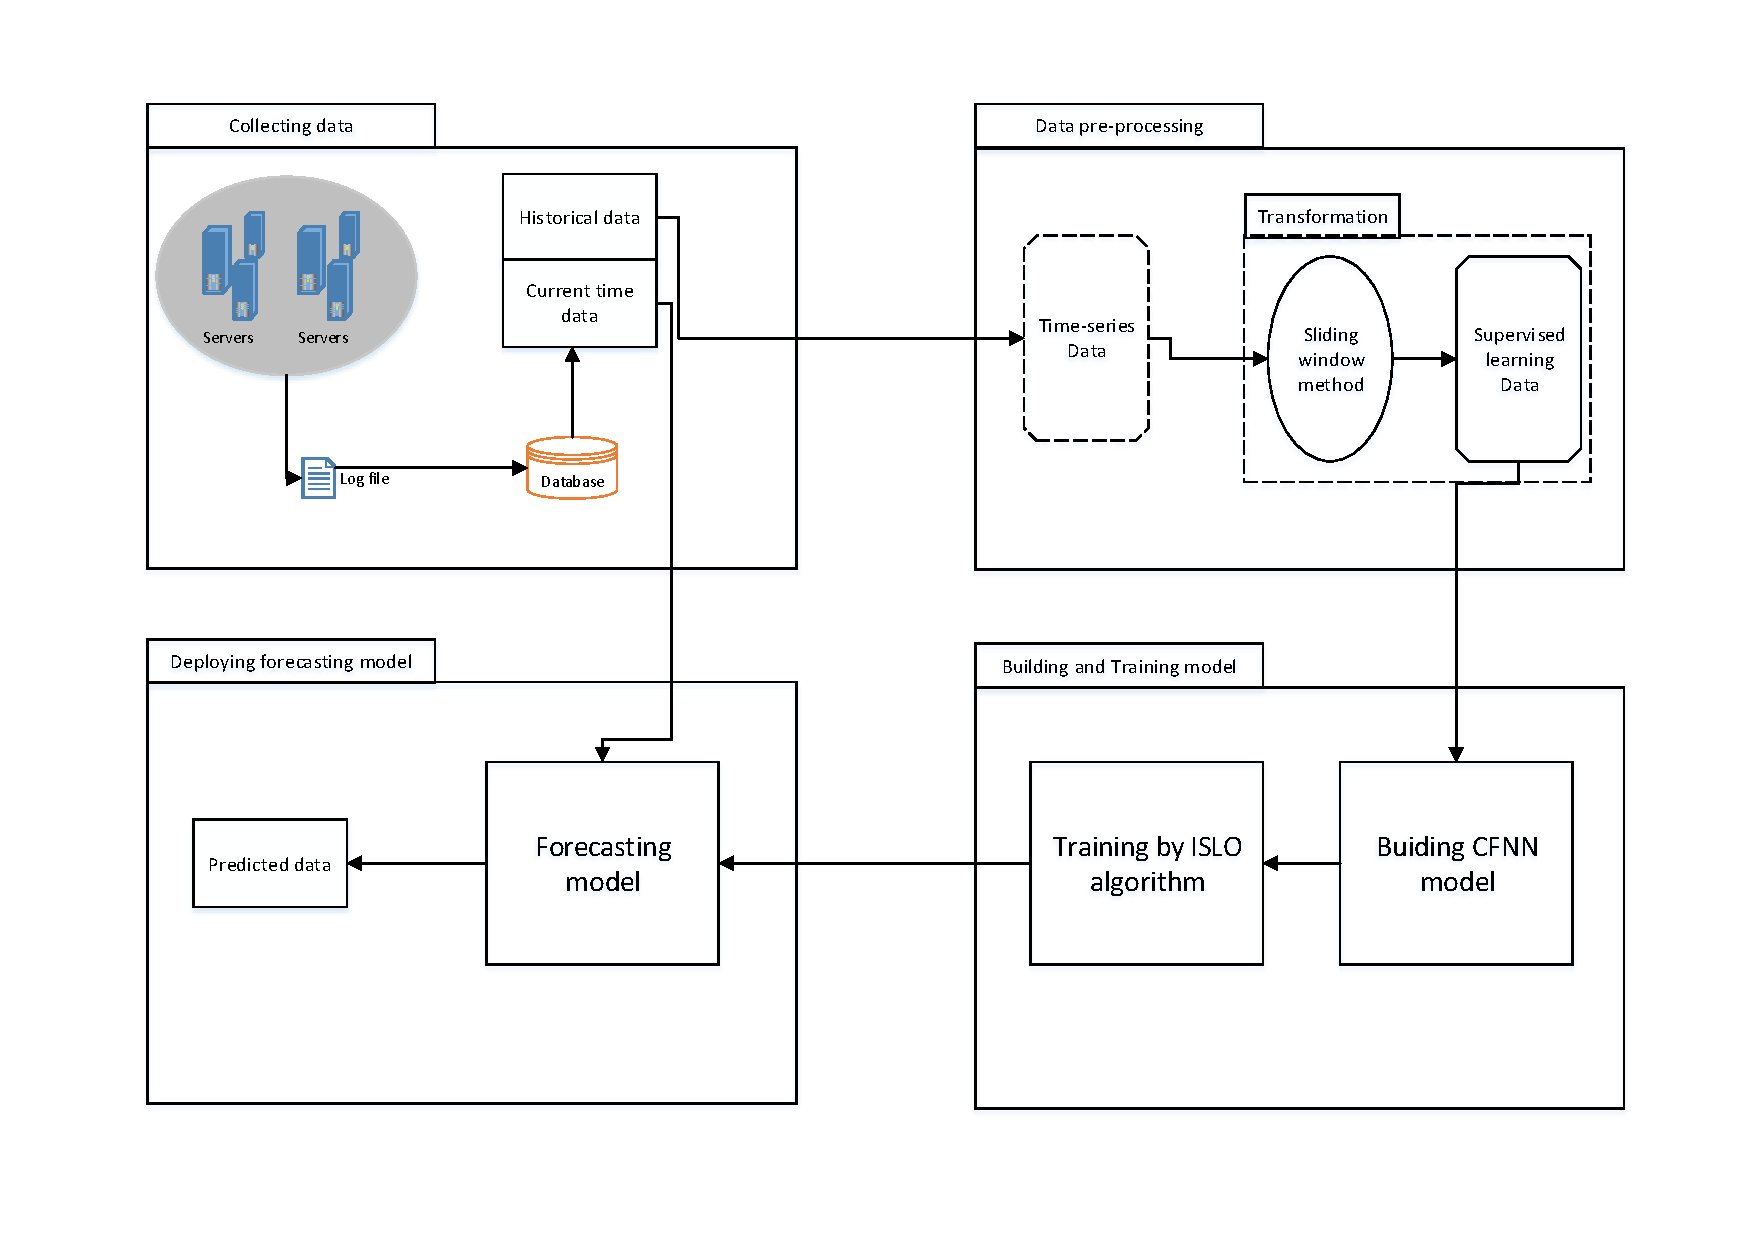
\includegraphics[width=1.0\linewidth]{/pdf/model/model_phases}
  \caption{Proposed model design} 
  \label{fig_model_phases} 
\end{figure}
	
\subsection{Collecting data}
\label{collect_data}
	
	Before building any forecasting systems, the very first and the most important task that must be done is collecting data. Therefore, we collect data recording the resource usage of Google (Google Cluster Trace data) and Internet Traffic data collected from a private internet service provider (ISP) in Europe and the United Kingdom (these datasets  will be discuss in detail in Chapter \ref{ch:experiments}. The data collected contains two main parts: the data from history that we use for training, and current time data that we use for predicting resource usage in the future.  
	

\subsection{Data pre-processing}
\label{data-pre}

\begin{table}[!t]
\caption{Time-series data and Supervised learning data comparison}
\label{tbl_data_cmp}
\centering
\begin{tabular}{|p{5cm}|p{5cm}|}
 \hline
 Time-series data & Supervised Learning data  \\ 
 \hline
 1. Time 1, value 1 & 1. Input 1, output 1  \\ 
 2. Time 2, value 2 & 2. Input 2, output 2  \\ 
 3. Time 3, value 3 & 3. Input 3, output 3  \\ 
 \hline
\end{tabular}
\end{table}
	
	This phase play a role as a pre-processor transforming the raw data into the kind of data that can be used in neural networks. In order to learn, models need both training data and testing data. We create the data for models through several steps as follows:

\begin{itemize}
\item  Evaluate and choose carefully which columns of data are needed for the forecasting model.
\item  The parts of data chosen are then normalized in the range $[ \, 0, 1 ] \,$.
\item Transform time-series data into supervised learning data using \textit{Sliding window} technique.
\item Divide processed data into two sets: training set and testing set.
\end{itemize}

	The step $3th$ of the pre-processing phase is necessary because time-series data is the data recorded through time, and there is no term of features and output data. Therefore, we need to transform this data into supervised learning data, that contains input features, and output. Table \ref{tbl_data_cmp} depicts the difference between time-series data and normal data used in supervised learning.


	In order to create data for supervised learning, we use the method called \textit{Sliding window}. This method takes the data of $k$ values before the time $t$ as the features and output data is the value at the time $t$. For example, when $k=3$, the results of data transformation is shown as in Table \ref{tbl_sliding_window}.
	
\begin{table}[!t]
\caption{Example of data transformation using Sliding window method}
\label{tbl_sliding_window}
\centering
\begin{tabular}{|p{4cm}|p{1.5cm}|p{1.5cm}|p{1.5cm}|p{1.5cm}|}
 \hline
 \multicolumn{1}{|c|}{Time-series data} & \multicolumn{4}{c|}{Transformed data} \\ 
 \hline
 \multicolumn{1}{|c}{} & \multicolumn{3}{|c}{Input} & \multicolumn{1}{|c|}{Output} \\
 \hline
  Time $(t=4)$, Value 4 & Value 1 & Value 2 & Value 3 & Value 4 \\
  Time $(t=5)$, Value 5 & Value 2 & Value 3 & Value 4 & Value 5 \\
  Time $(t=6)$, Value 6 & Value 3 & Value 4 & Value 5 & Value 6 \\
  Time $(t=7)$, Value 7 & Value 4 & Value 5 & Value 6 & Value 7 \\
 ... & ... & ... & ...  & ... \\
 \hline
\end{tabular}
\end{table}	
	 
\subsection{Building and Training model}
\label{main_model}

	In this phase, pre-processed data is used for training our proposed model called ISLO-CFNN, which is CFNN being trained by the optimization of ISLO algorithm. ISLO algorithm is applied to train a CFNN model with one hidden layer. There is two key aspects needed to be taken into consideration: firstly, the formation of an agent in ISLO and the selection of fitness function.
	
	Firstly, each agent in the population in ISLO are presented as one solution for CFNN model, which means that a search agent is a one-dimensional vector created by concatenating weights and biases of CFNN. Therefore, the features of a search agent contains three elements: a set of weights connecting the input layer with hidden layer, a set of weights connecting the hidden layer with output layer and also and a set of weights connecting the input layer with output layer. Therefore,  the length of a solution can be calculated by Eq. \ref{eq_length_solution}.	
\begin{equation} \label{eq_length_solution}
	Solution\_length = (1+i)*h + (1+h)*o + (1+i)*o
\end{equation}
Where $i, h, o$ is the number of input, hidden and output neurons,  respectively (in time-series prediction, the number of output neurons is one).
\begin{figure}[!ht] 
   \centering
   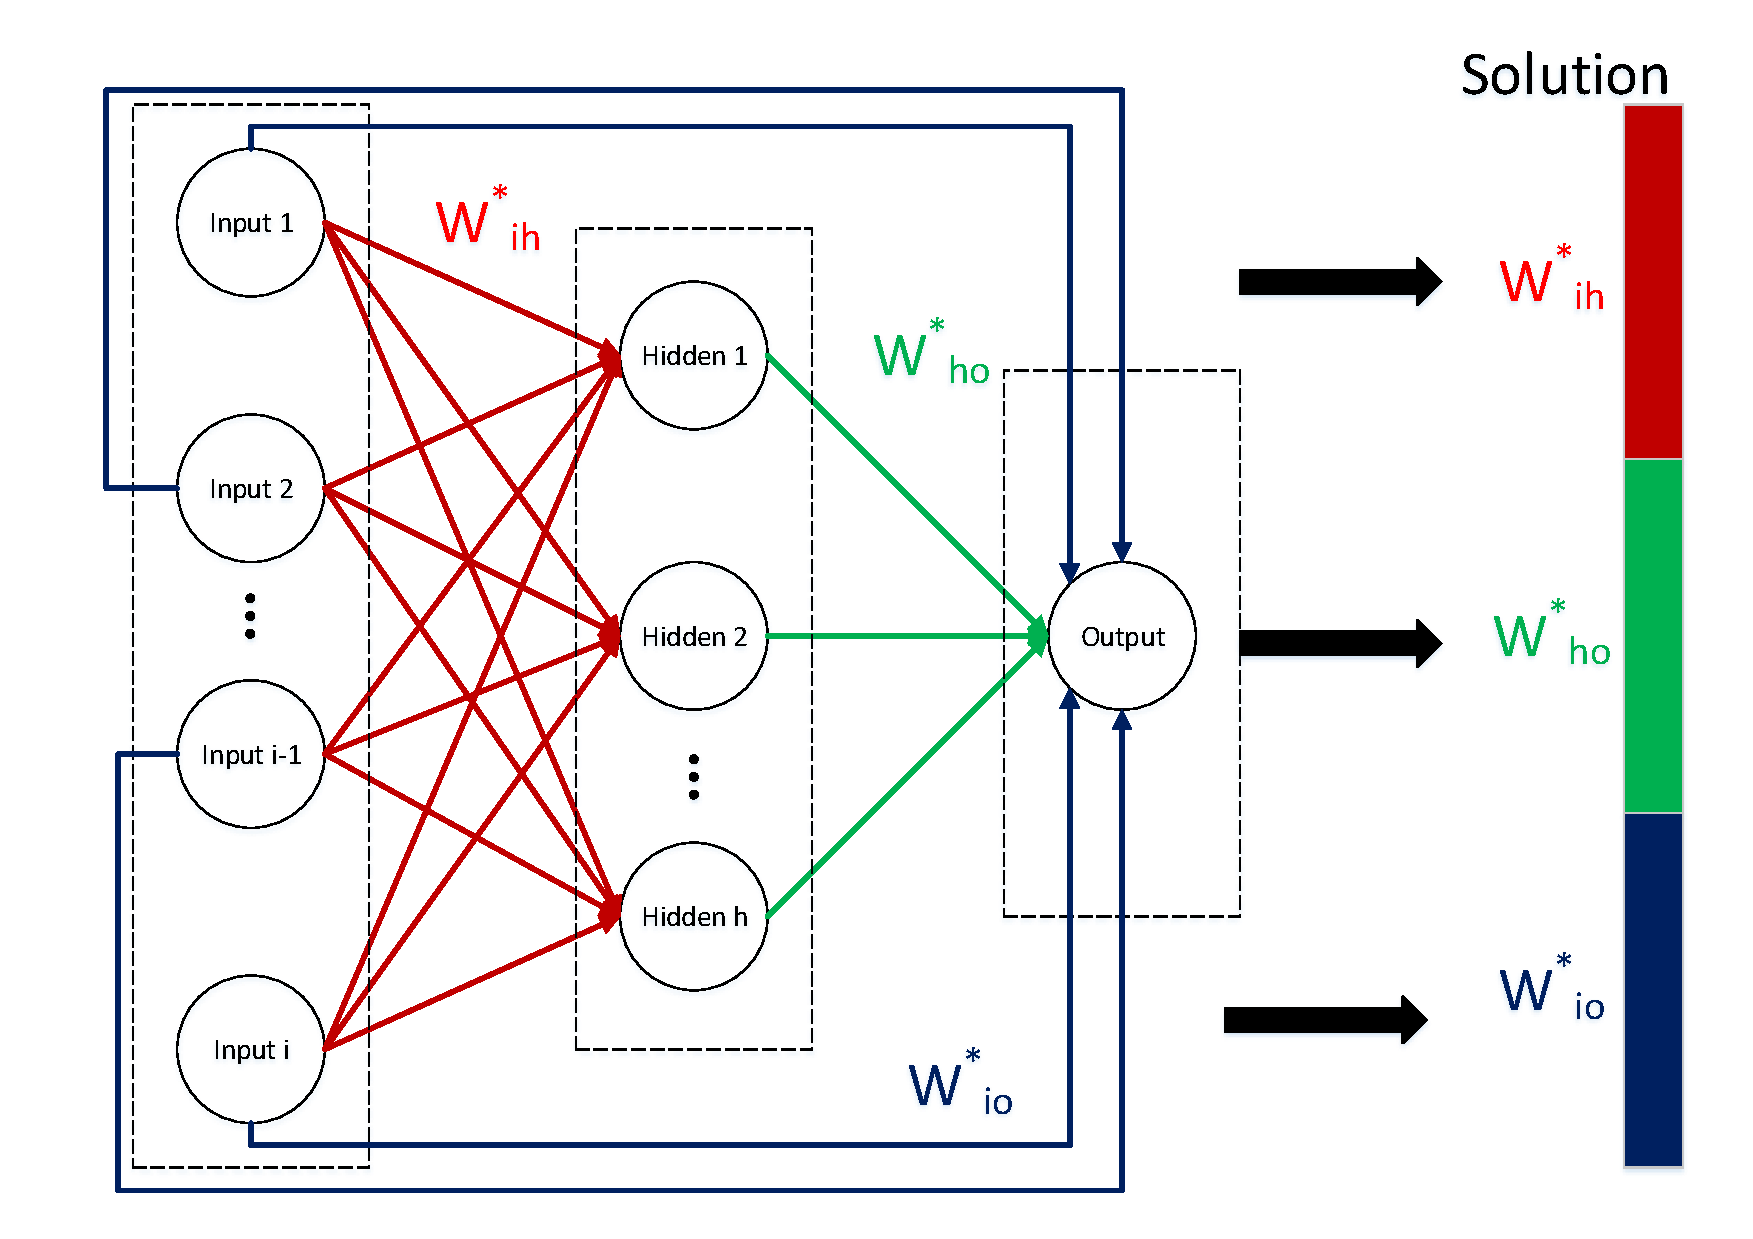
\includegraphics[width=0.75\linewidth]{pdf/model/solution_creation}
  \caption{Encoding process transforming a parameter set in CFNN into an agent in ISLO algorithm. ($W^*$ indicates weights and biases between 2 layers)} 
  \label{fig_solution_encode} 
\end{figure}
	
	Secondly, the fitness value of each agent in ISLO is considered as the loss value of the CFNN model with the parameter set from the agent and input data. We utilize the loss function Mean Square Error (MSE) to calculate the difference between the actual and predicted output values by generated agent for all samples in the training set. 
\begin{figure}[!ht] 
   \centering
   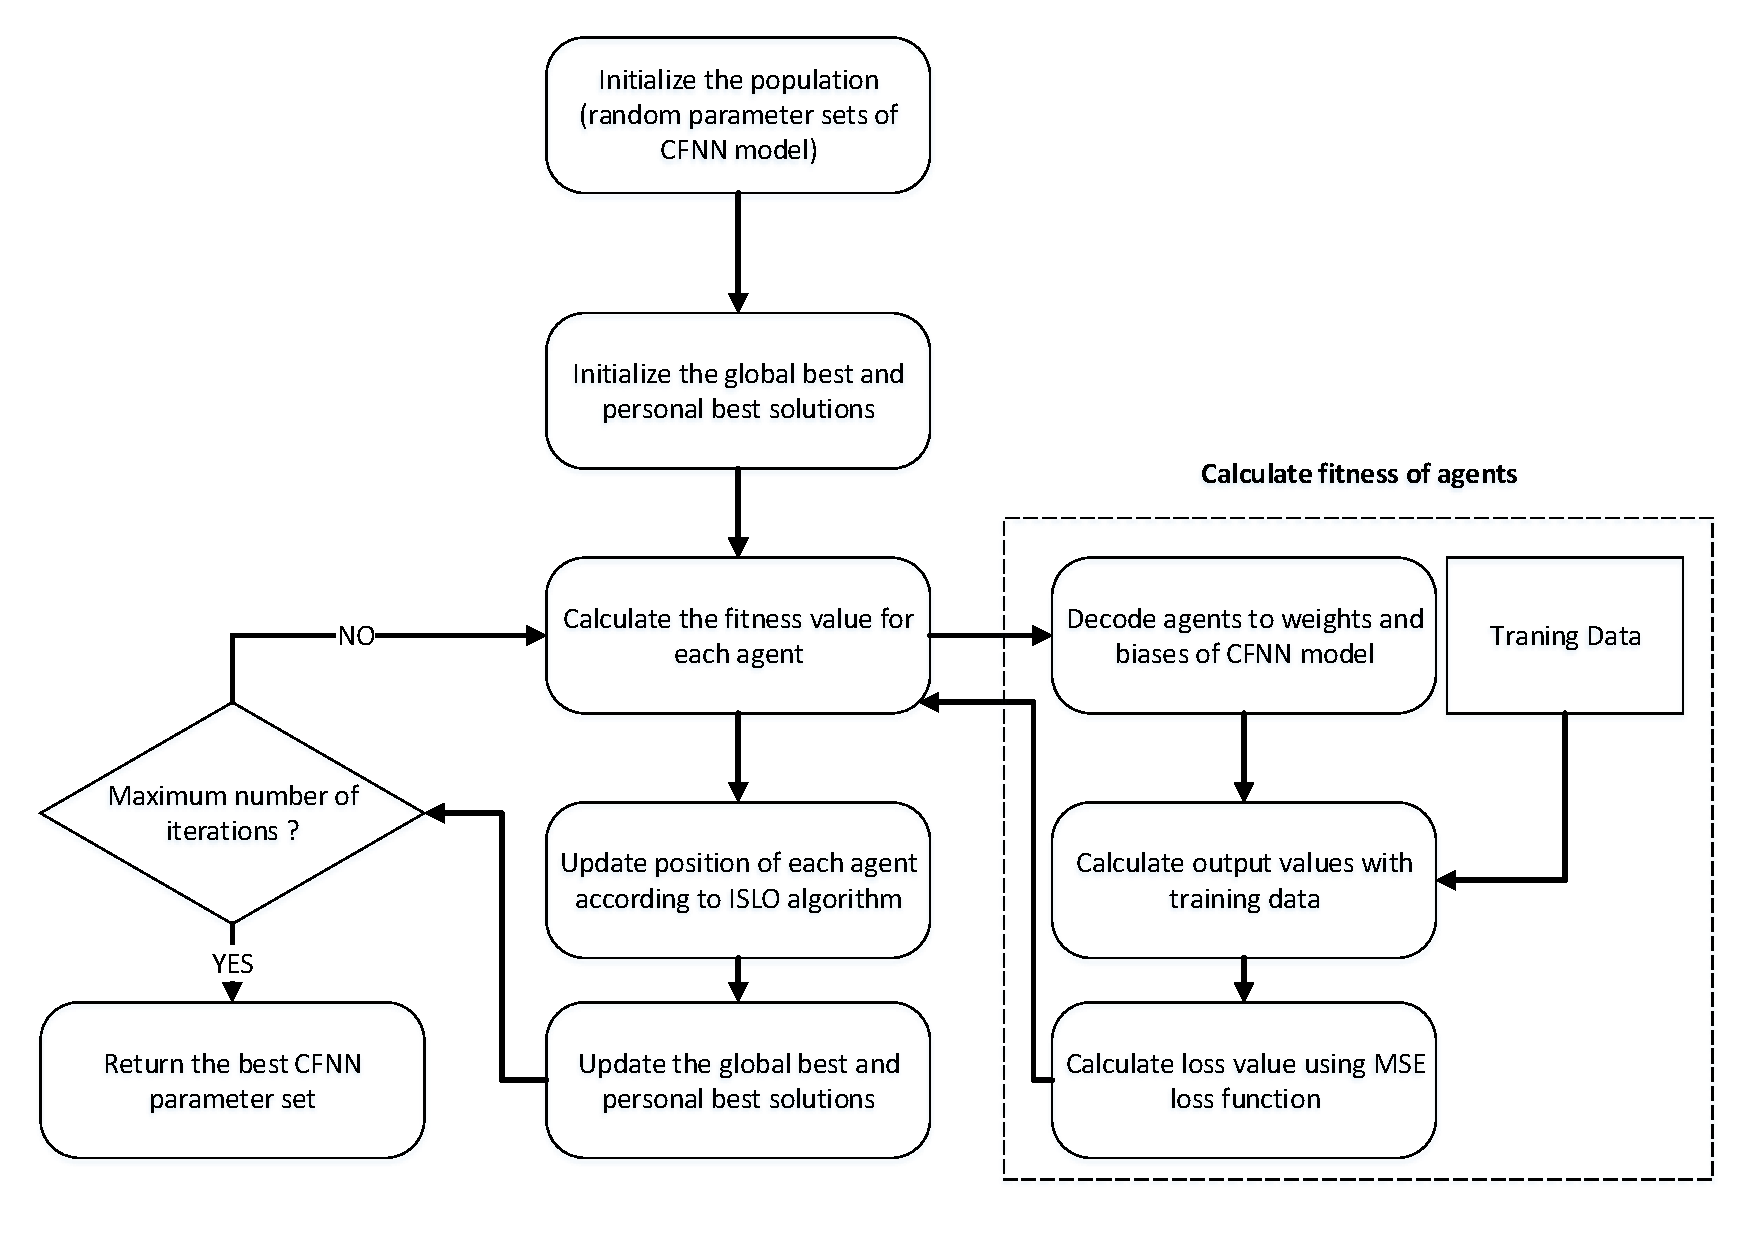
\includegraphics[width=1.0\linewidth]{pdf/model/islo_cfnn_workflow}
  \caption{The work flow of ISLO-CFNN model.} 
  \label{fig_islo_cfnn_workflow} 
\end{figure}	

	The workflow of ISLO applied in this work for training CFNN are depicted in Fig. \ref{fig_islo_cfnn_workflow}, and can be generally presented by the following steps:
	
\begin{enumerate}
\item Initialization: pre-define the number of search agents in ISLO, which are randomly generated in the range [-1, 1]. Each parameter set of CFNN model is encoded to a vector playing a role as an agent in ISLO population. (See in Fig. \ref{fig_solution_encode})
\item Calculate fitness value for each search agent: The quality of a solution is measured by the loss value of CFNN output. After being decoded into weights and biases vectors, a solution will be applied to form a CFNN model. Data samples in training set is then feed-forwarded through the network, generating predicted output values. Finally, the fitness value is calculated as the difference between predicted and actual output values through the MSE loss function.
\item Update positions of all search agents following formulas of ISLO algorithm.
\item Steps 2 and 3 are repeated until the difference is close enough, or the maximum number of iterations is reached.
\item Return the best CFNN parameter set. 
\end{enumerate}
	     
\subsection{Deploy prediction model}
\label{deploy}
	
	After obtaining CFNN model with the best parameter set by ISLO algorithm, the model is installed on servers and ready to predict the demand for resources in the future based on historical data.


\section{Chapter conclusion}
	
	In this chapter, we propose ISLO algorithm with two improvements on the original SLnO algorithm. One of them is based on the idea of PSO algorithm, taking individuals' best position into consideration for enhancing exploitation phase, and another is choosing new random agent following the OBL technique for the increase in the diversity of population. Furthermore, proposed ISLO algorithm is applied to optimizing Cascade Feedforward Neural Network (CFNN), forming ISLO-CFNN model. This model is introduced for tackling the time-series prediction problem, especially workload prediction in cloud computing.
\end{document}